\documentclass{article}

%% Preamble

\usepackage[margin=1in]{geometry}
\usepackage{graphicx}
\usepackage{amsmath}


\title{Global Suicide Rate Study}
\author{Zach Drane}
\date{December 28, 2020}

\begin{document}

\section{Abstract}
\(\text{ } \)

I found a dataset to analyze from Kaggle at \\
\noindent \emph{https://www.kaggle.com/russellyates88/suicide-rates-overview-1985-to-2016}\\
The data was pulled from four different sources. The United
Nations Development program, The World Bank, a second kaggle
dataset, and the World Health Organization. I was curious to see
which factors contributed to higher suicide rates. From this
dataset, there doesn't seem to be a direct link between
GDP per capita and suicide rates. The strongest predictors of
suicide rates were sex and age.

\section{Results}

The relation between the GDP per capita and the suicide rates was surprising. I expected
to see more suicides in less wealthy nations due to harsher living conditions. The data
shows that the correlation is very weak. The linear model shows an \(R^2\) value of only
\(-0.0086\).
Figure~1 %\ref{fig::gdp}
shows a scatter plot of gdp against suicide rates.

\begin{figure}[h!]\centering
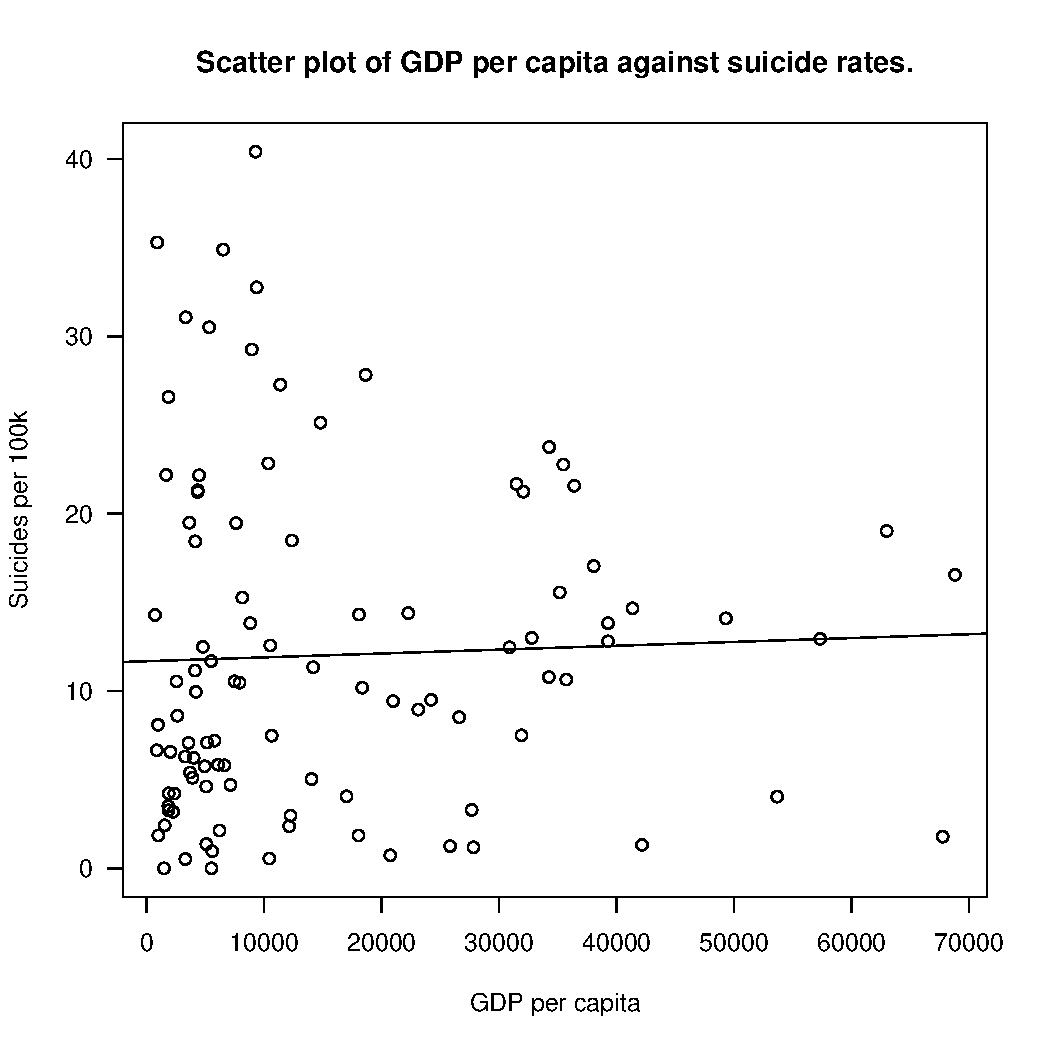
\includegraphics[width=0.5\textwidth]{sui-by-gdp.pdf}
\label{fig::gdp}
\caption{}
\end{figure}

The relationship between birth sex and suicide rates was much more significant.
The mean suicide rate for males was \(17.50\) with a standard deviation of \(14.53\),
but the mean suicide rate for females was only \(4.88\) with a standard deviation of \(3.91\).
The extreme standard deviation for male suicide rates makes it more difficult to determine
the true mean of male suicde rates. We can be confident that the true mean for male
suicides is between \(14.63 \text{ and } 20.37\). By contrast, we can be \(95\%\) confident
that the true mean for female suicide rates is between \( 4.11 \text{ and } 5.66 \).
A t test confirms that this value difference is significant with a
p value of $6.161 * 10^{-14}$. Figure~2 %\ref{fig::sex}
displays the difference.

\begin{figure}[h!]
\centering
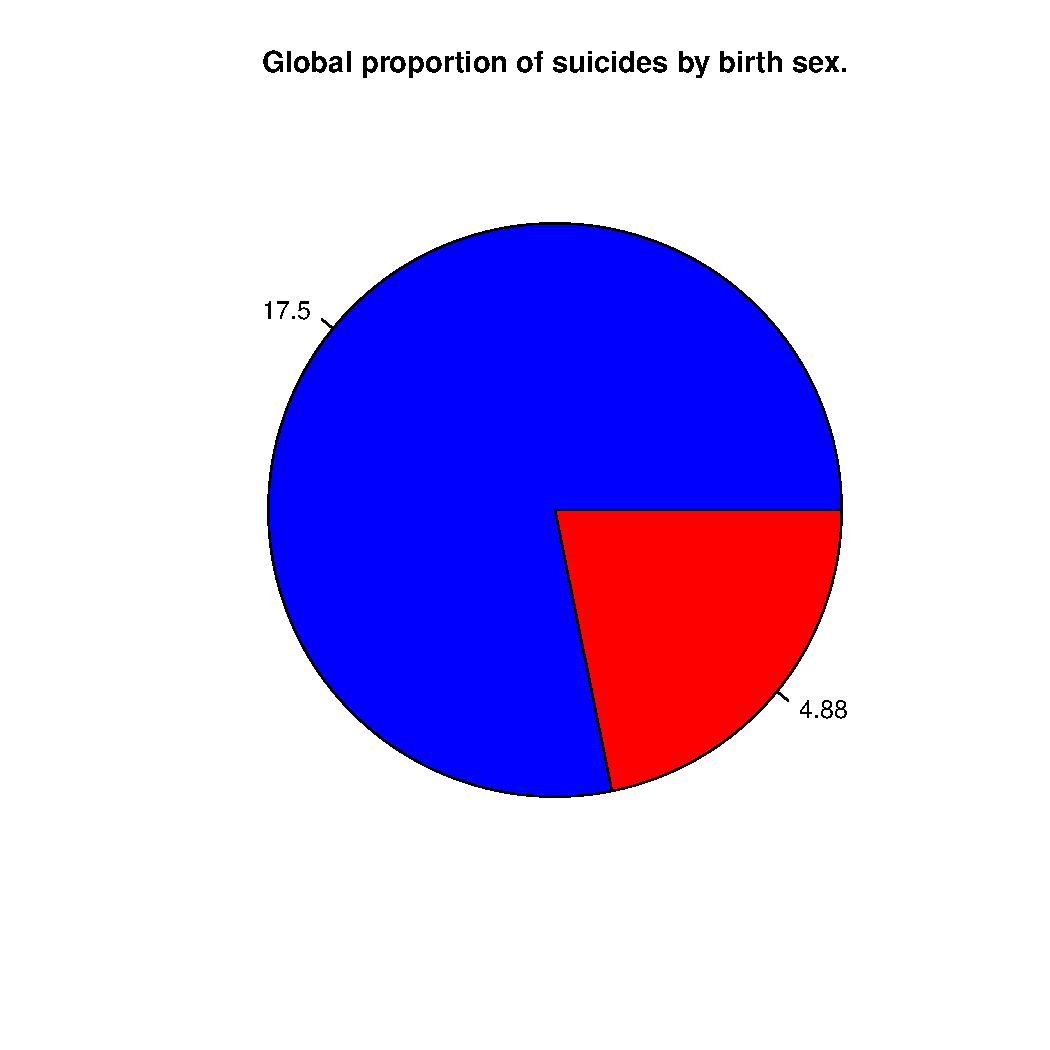
\includegraphics[width=0.5\textwidth]{sui-by-sex.pdf}
\label{fig::sex}
\caption{}
\end{figure}

Splitting the data into \(6\) different age groups yields interesting results. The
data seems to indicate an increasing suicide rate with increasing age, but running an
ANOVA test indicates that we have insufficient evidence to conclude this. The p value
for the ANOVA is only \(0.572\). Figure~3 %\ref{fig::age}
shows a graph of the suicide rates
broken down into age categories.

\begin{figure}[h!]
\centering
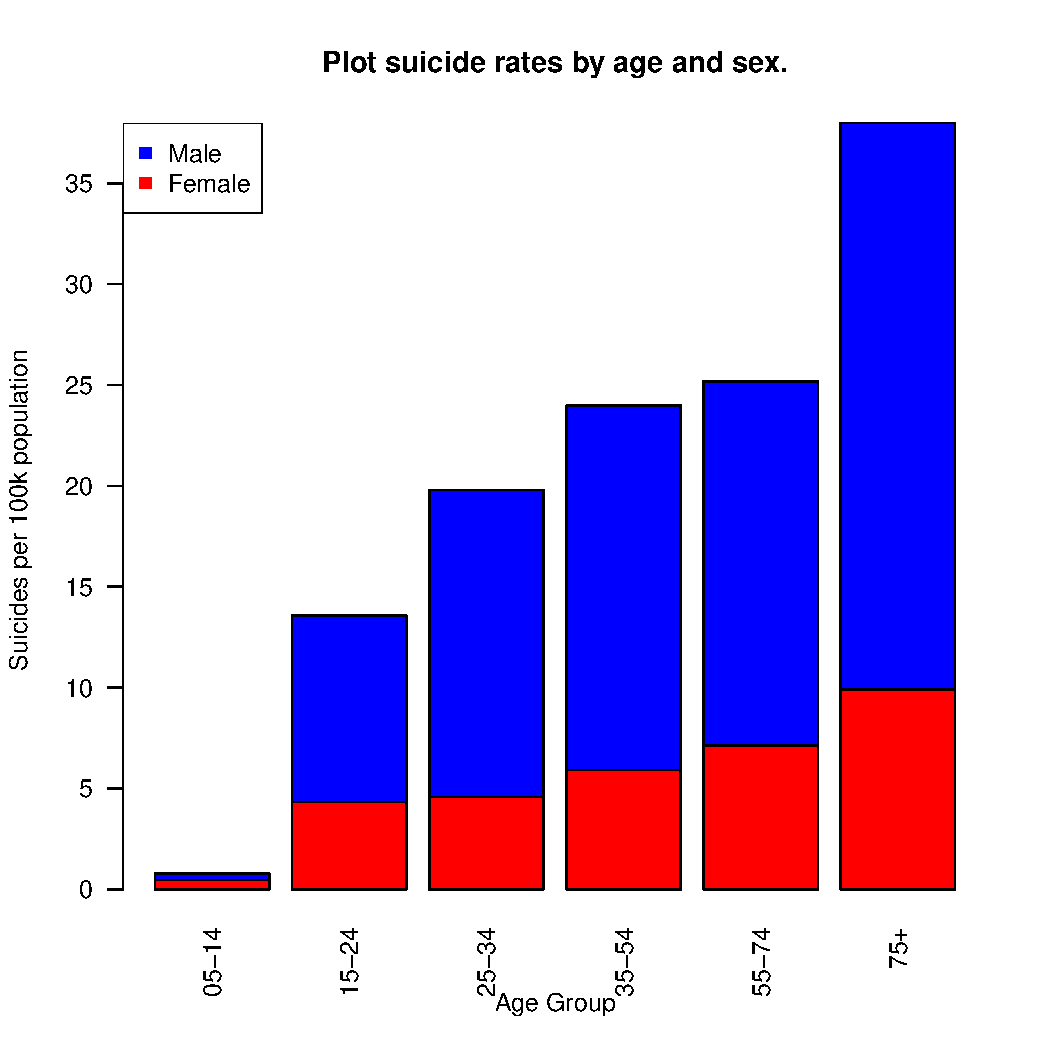
\includegraphics[width=0.5\textwidth]{sui-by-age-by-sex.pdf}
\label{fig::age}
\caption{}
\end{figure}




\end{document}
